% !Mode:: "TeX:UTF-8"
% !TEX root = ..\thesis.tex
\chapter{多品种装配车间调度建模}
本章将对装配线生产进行分析,指出现有计划安排和调度存在的主要问题,然后针对这些问题,提出合理解决方案,并对其进行分析和数学建模。



上述问题为研究对象的目前的主要问题,并对其产生原因进行分析,这为改进调度方案明确了方向。具体改进过程需要通过建模分析。

\section{建模准备}
为制定合理调度方案,改善装配流水线现状,首先需要确定改进目标,进而根据目标的可行性,建立数学模型。
因此,本节将结合实际情况,权衡投入和效益,建立适合本课题研究对象的混线装配生产模型。
\subsection{目标设计}
目前的生产现状主要是存在各主机厂的专用流水线,所以首要的改进是突破专用线的生产界限。如此一来,生产线可以加工多家主机厂的订单,形成所谓的混线生产,是较混流生产为宏观的均衡化生产,如\reff{fig:orderschedule}所示\footnote{\reff{fig:orderschedule}中订单a -- b 表示主机厂a 的第b 个订单}
。其次,适当允许任务中断,安排插单作业,可以近一步改善现有浪费,而且增加生产应变能力。
\begin{figure}[h]
\centering
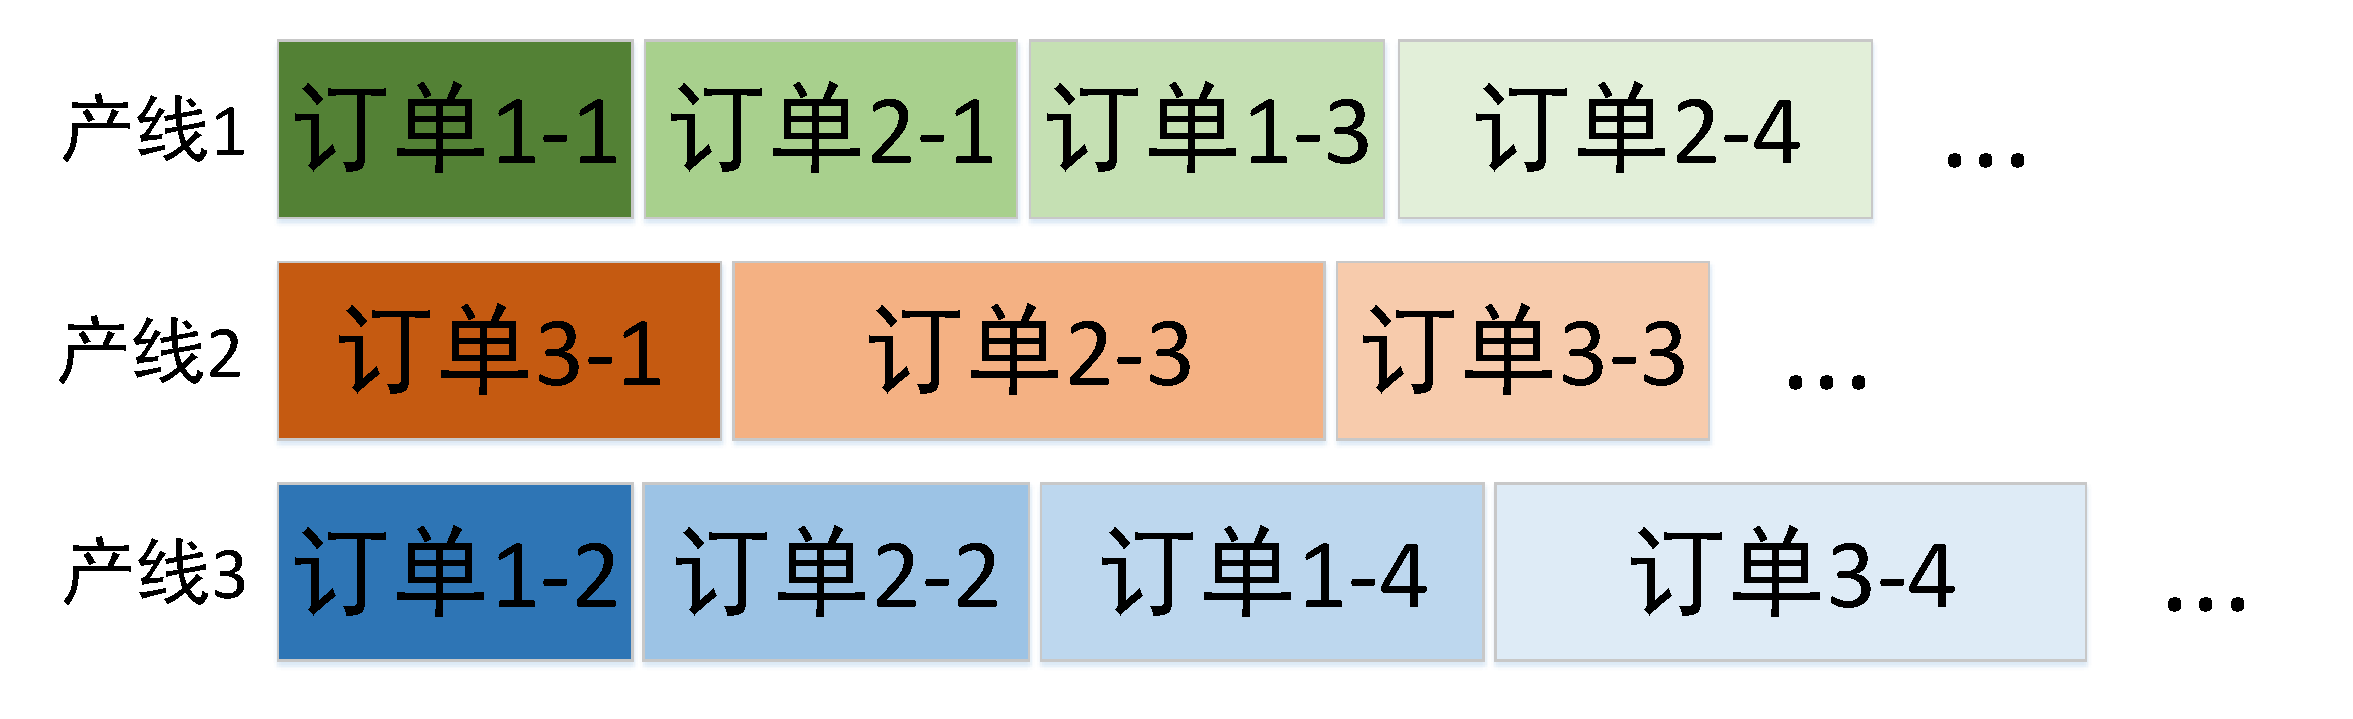
\includegraphics[width = 8cm]{oredrschedule.pdf}
\caption{3条产线的混线装配生产示意\label{fig:orderschedule}}
\end{figure}

根据这样的目标,对所需生产的订单进行排列组合,较为均匀地安排在各流水线上,以期获得均衡的生产线利用率、减少换线时间浪费、缩短完工时间、降低生产成本。此外,虽然实施完全均衡化生产需要有较高的管理水平和投入,但是适当的混流(即考虑投入产出关系后)可以有效提高产线性能,需要确定混流程度。

产品订单确定其所需产品的数量(订单批量),订单中的每个产品可以看作为作业,流水线上的各装配工位或机器看作处理单元,由于本课题的研究主要内容较少涉及具体的装配工艺,故产品订单也确定了作业处理所需的处理单元的数量、种类以及顺序,流水线上的订单处理可以看作是各作业按固定顺序经过线上的处理单元进行处理。

\subsection{基本符号说明}
为了方便问题描述,需要说明基本符号如下,其中涉及的时间变量研究对象为系统时间:

\begin{supertabular}{ll}
$n$ & 订单数量\\
$m$ & 流水线数量\\
$j$ & 订单标记,$j = 1,2,...,n$\\
$N$ & 所有订单集合\\
$l$ & 流水线标记,$l = 1,2,...,m$\\
$S_l$ & 流水线$l$上的订单调度\\
$|S|$ & 调度$S$的订单数量\\
$\overline S$ & 调度$S$中的订单集合\\
$l_k$ & 调度$S_l$的第$k$项订单标记,,$k = 1,2,...,|S|$\\
$d_j$ & 订单$j$的交货时刻(工期)\\
$t$ & 生产系统时间\\[3pt]
\end{supertabular}

一个调度问题可以由三元组$\alpha \mid \beta \mid \gamma$表示,$\alpha$域描述单一处理单元环境,$\beta$域包含加工特征和约束的细节,$\gamma$域描述其目标\cite{pinedo}。

\subsubsection{基本$\alpha$域}
\begin{supertabular}{ll}
$Pm$ & 并行同速并行机\\
$Fm$ & 流水车间\\
\end{supertabular}

\subsubsection{基本$\beta$域}
\begin{supertabular}{ll}
$r_j$ & 订单$j$进入流水线系统日期,是其最早可开始时刻\\
$s_j$ & 订单$j$开始之前所需的切换(开工)准备时间\\
\end{supertabular}

\subsubsection{基本$\gamma$域}
$\gamma$域涉及目标函数,一般调度问题需要考虑最小化目标函数,常见的目标函数为订单$j$的完成时刻$C_j$,为订单$j$离开系统的时刻。订单$j$的迟滞可以定义为:
\[
L_j = C_j - d_j
\]
进一步可定义其延迟和提前:
\begin{align*}
T_j & = \max(L_j,0)\\
E_j & = \max(-L_j,0)
\end{align*}
常见基本$\gamma$域有:\\[3pt]
\begin{supertabular}{ll}
$\sum w_jC_j$ & 加权订单完成时刻总和 \\
$\sum w_jT_j$ & 加权订单延迟时间总和 \\
%$\sum w_jE_j$ & 加权订单提前时间总和
\end{supertabular}

\section{基本模型}
\subsection{基本假设}
假设订单、订单包含的作业、订单涉及的处理单元以及流水线数量有限,
订单中的每项作业均相同,相同处理单元布置在不同流水线上的处理能力不变,也就是说同订单中的作业在不同流水线的处理时刻相同。
所有订单在系统时刻$t = 0$时下达,皆可开始生产处理,即$\forall r_j =0$,并且之后没有新的订单进入系统。
处理过程中,订单不可被中断,即订单一旦开始装配处理,就要不间断地处理完整个批量。
由于该厂总装厂的产品体积较小,可以忽略生产线上处理单元间的在制品
本课题的调度研究不涉及具体的装配工艺流程,故假定不同产品的工艺区别只能体现在处理时间和设备准备时间,
按队列生产时,处理不同订单需要考虑切换准备时间,切换准备时间只和订单本身有关,并且所需准备时间事先已知。此外,各流水线除了切换准备一般不停线等待。
所有作业均完成的订单方可交付

\subsection{目标函数}
本课题期望通过合理调度,达到提高产线利用率、减少浪费、缩短制造期、提高应变能力、减少库存、降低生产成本等目标,这些目标有着内在联系,所以在设计目标函数的时候,不必把每样都列入其中,比如最小化完成时刻在一定程度上相当于最大化处理单元利用率,进一步可以暗示最大化流水线利用率。

对于基本模型,可以考虑满足工期和提高产线利用率,其中满足工期为主要目标,可用加权延迟时间和$\sum wt_jT_j$;产线利用率为次要目标,可用加权完成总时刻和$\sum wc_jC_j$。其中$wt_j, wc_j$分别为订单$j$的延迟和完工权重。

进一步分析该问题,可以发现由给出的基本假设订单不可中断,那么每个订单的总装配生产时间是确定的,并且与其被加工的流水线无关,所以可将各装配线看作是并行同速机环境,每条产线看作一个可以处理所有订单的机器。该问题可以记为:$Pm \mid s_j\mid\sum wt_jT_j(\text{opt}), \sum wc_jC_j$\ ,那么该目标函数可表示为:

\begin{equation}
\min\quad \sum_{j = 1}^n wt_jT_j(\text{opt}), \sum_{j=1}^n wc_jC_j
\label{equ:primeobj}
\end{equation}

表示在主要目标(opt)达到最优的所有调度中,搜寻出使次要目标最小化的调度方案,一般来说,对换主次目标得到的调度方案不同。根据\eqref{equ:primeobj}中主要目标的特性,并从产线角度来考虑,可以改写成如下等价形式:
\begin{equation}
\min\quad \sum_{l=1}^m\sum_{k=1}^{|S_l|} wt_{l_k}T_{l_k}
\label{equ:objmain}
\end{equation}
同理,\eqref{equ:primeobj}的次要目标函数可改写成:
\begin{equation}
\min\quad \sum_{l=1}^m\sum_{k=1}^{|S_l|}wc_{l_k}C_{l_k}\label{equ:objsecond}
\end{equation}
\subsubsection{约束条件}
约束条件需要从订单间的关系中寻找,
并行机环境中,可以根据产线来考虑订单。记订单$l_k$的处理时间为$p'_{l_k}$,由于其准备时间为定值$s_{l_k}$,可以将其并入订单处理时间来简化问题而不影响结果,并记订单$l_k$的整合切换准备处理时间为$p_{l_k}$,那么该基本模型的主要约束如下:
\begin{numcases}{}
\sum_{l=1}^m |S_l| = n\label{equ:basicst1}\\
\bigcup_{l=1}^m \overline{S_l} = N\label{equ:basicst2}\\
C_{l_1} = p_{l_1} & $l = 1,2,...,m$\label{equ:basicst3}\\
C_{l_k} = C_{l_{k-1}} + p_{l_k} & $k = 2,3,...,|S_l|, l = 1,2,...,m$\label{equ:basicst4}\\
p_{l_k} = p'_{l_k} + s_{l_k} & $k = 1,2,...,|S_l|, l = 1,2,...,m$\label{equ:basicst5}\\
T_{l_k} = \max(0, C_{l_k} - d_{l_k}) & $k = 1,2,...,|S_l|, l = 1,2,...,m$\label{equ:basicst6}\\
p'_{l_k}, s_{l_k}, d_{l_k}, wt_{l_k}\ge 0 & $k = 1,2,...,|S_l|, l = 1,2,...,m$\label{equ:basicst7}
\end{numcases}



\section{插单模型}
插单模型考虑系统在开始运行后,有新的订单进入系统,需要对其进行调度安排。这是比较符合实际的情况。

\subsection{相关符号及说明}
在基本模型基础上,需要补充或修改符号定义如下:


\subsection{相关假设}
根据订单到达先后动态安排调度的难度较大,而且也难以实施应用,故可以假设所有订单在$t=0$时皆已知,插单相当于指定了某订单的最早可开始时间,即$\exists r_{l_k} >0$。
系统时间由订单情况而定,假定系统从开始换线为时间起始,即要保证$\min(r_{l_k}) = 0$,需要进一步处理,记各订单进入流水线时间为$r'_{l_k}$,则变换后的进入系统时间为$r_{l_k} = r'_{l_k} - \min(r'_{l_k})$。
需假设所有订单不可被中断

\subsection{目标函数}
考虑插单时,更为注重订单的按时交付,同时也关注产线利用率,所以其主要目标和次要目标和基本模型一致,那么插单模型的调度可以表示为:
$Pm\mid r_j, s_j\mid\sum wt_jT_j(\text{opt}), \sum wc_jC_j $。

主要目标函数为:
\begin{equation}
\min\quad \sum_{l=1}^m\sum_{k=1}^{|S_l|} wt_{l_k}T_{l_k}
\label{equ:insertobjmain}
\end{equation}
次要目标函数为:
\begin{equation}
\min\quad \sum_{l=1}^m\sum_{k=1}^{|S_l|}wc_{l_k}C_{l_k}\label{equ:insertobjsecond}
\end{equation}
\subsection{约束条件}
插单模型是以基本模型为基础,需要多考虑订单进入时刻,所以要对基本约束进行修改和增加:
\begin{numcases}{}
\sum_{l=1}^m |S_l| = n\label{equ:insertst1}\\
\bigcup_{l=1}^m \overline{S_l} = N\label{equ:insertst2}\\
C_{l_1} = p_{l_1} + r_{l_1}& $l = 1,2,...,m$\label{equ:insertst3}\\
C_{l_k} = \max(C_{l_{k-1}}, r_{l_k}) + p_{l_k} & $k = 2,3,...,|S_l|, l = 1,2,...,m$\label{equ:insertst4}\\
p_{l_k} = p'_{l_k} + s_{l_k} & $k = 1,2,...,|S_l|, l = 1,2,...,m$\label{equ:insertst5}\\
\sum_{l=1}^m\sum_{k=1}^{|S_l|} r_{l_k} > 0& $k = 2,3,...,|S_l|, l = 1,2,...,m$\label{equ:insertst6}\\
T_{l_k} = \max(0, C_{l_k} - d_{l_k}) & $k = 1,2,...,|S_l|, l = 1,2,...,m$\label{equ:insertst7}\\
p'_{l_k}, s_{l_k}, d_{l_k}, wt_{l_k}, r_{l_k}\ge 0 & $k = 1,2,...,|S_l|, l = 1,2,...,m$\label{equ:insertst8}
\end{numcases}

\section{分单模型}
在基本假设中,订单一旦开始装配处理,就要不间断地处理完整个批量,然而这样的生产安排必然对提高产线利用率不利。考虑将订单拆分,将订单的作业分布在各流水线上,可以提高产线利用率,然而由于需要考虑切换准备,并不是拆分越多越好。此外,先前订单的完成时刻不再为定值,所以另外还需要设计其求解方法,这将在下一章中具体分析。
\subsection{相关符号及说明}
在基本模型基础上,需要补充或修改符号定义如下:\\[3pt]
\begin{supertabular}{ll}
$n_j$ & 订单$j$的作业(需求)量\\
$n_{j,l}$ & 订单$j$分配在流水线$l$上的作业数量\\
$p_{j,l}$ & 订单$j$分配在流水线$l$上的子单处理时间\\
$s_{k,l}$ & 订单$j$分配在流水线$l$上的子单切换准备时间\\
$C_{j,l}$ & 订单$j$分配在流水线$l$上的子单完成时刻\\
\end{supertabular}

\subsection{相关假设}
在基本假设基础上,考虑各订单可以拆分的情况,需要进行一些假设补充。
考虑插单时,拆分的最小单元为订单中的作业,并称分出的订单为子单,每条流水线至多分配到某订单的一个子单。
订单$j$的完成时刻$C_j$为该订单中最后一个离开系统的作业的时刻,若订单$j$没有在流水线$l$上分配子单,那么$C_{j,l} = 0$。
各子单开始前都需进行切换准备,其准备时间为所属订单的切换准备时间,即$s_{j,l} = s_j$。
子单在流水线上的处理时间无产线差别,只和其作业数量及处理单元有关。
\subsection{目标函数}
分单的目的是为了使装配生产更为均衡化,提高产线利用率,而且这么操作满足较为容易工期,故以加权完成时刻为主要目标,并以加权延迟时间和为次要目标,那么该模型的调度问题可记作:
$Pm\mid s_j\mid \sum wc_jC_j(\text{opt}), \sum wt_jT_j$
主要目标函数为:
\begin{equation}
\min\quad \sum_{j = 1}^n  wc_jC_j
\label{equ:apartmainobj}
\end{equation}
次要目标函数为:
\begin{equation}
\min\quad \sum_{j = 1}^n wt_jT_j
\label{equ:apartsecondobj}
\end{equation}
\subsection{约束条件}
在寻找约束前,需要对子单处理时间作一些说明。首先,子单处理时间可以这样求得:
\begin{equation}
p_{j,l} = f(j, n_{j,l})
\end{equation}
函数$f(j, n_{j,l})$将在下一章具体表述,同样,流水线上的订单标记可以另一个函数表示:
\begin{equation}
l_k = g(j, l)
\end{equation}
这样可用$p_{j,l}$确定$p_{l_k} = p_{g(j,l)}$及$s_{l_k} = s_{g(j,l)}$

分单模型以基本模型为基础,需要对基本约束进行增改。
\begin{numcases}{}
|S_l| \le n&$l = 1,2,...,m$\label{equ:apartst1}\\
\sum_{l=1}^mn_{j,l} = n_j & $j = 1,2,...,n$ \label{equ:apartst2}\\
C_{l_1} = s_{l_1} + p_{l_1} & $l = 1,2,...,m$\label{equ:apartst3}\\
C_{l_k} = C_{l_{k-1}} + s_{l_k} + p_{l_k} & $k = 2,3,...,|S_l|, l = 1,2,...,m$\label{equ:apartst4}\\
C_j = \max_{1\le l\le m}(C_{j,l}) & $j = 1,2,...,n$\label{equ:apartst5}\\
T_j = \max(0, C_j - d_j) & $j = 1,2,...,n$\label{equ:apartst6}\\
p_{l_k}, s_{l_k}, d_j, wt_{l_k}\ge 0 & $k = 1,2,...,|S_l|, l = 1,2,...,m, j = 1,2,...,n$\label{equ:apartst7}
\end{numcases}

\section{综合模型}
综合模型同时考虑插单和分单,主要以分单模型为基础,进一步考虑订单进入系统的时刻,更为符合实际情况。
\subsection{相关假设}
在分单模型的假设基础上,参考插单模型的假设。
所有订单在$t=0$时皆已知
同切换准备时间类似,各子单的进入系统时刻为所属订单的进入系统时刻,即$r_{j,l} = r_j$。
\subsection{目标函数}
\subsection{约束条件}
\begin{numcases}{}
|S_l| \le n&$l = 1,2,...,m$\label{equ:apartst1}\\
\sum_{l=1}^mn_{j,l} = n_j & $j = 1,2,...,n$ \label{equ:apartst2}\\
C_{l_1} = s_{l_1} + p_{l_1} & $l = 1,2,...,m$\label{equ:apartst3}\\
C_{l_k} = \max(C_{l_{k-1}}, r_{l_k}) + s_{l_k} + p_{l_k} & $k = 2,3,...,|S_l|, l = 1,2,...,m$\label{equ:apartst4}\\
C_j = \max_{1\le l\le m}(C_{j,l}) & $j = 1,2,...,n$\label{equ:apartst5}\\
T_j = \max(0, C_j - d_j) & $j = 1,2,...,n$\label{equ:apartst6}\\
p_{l_k}, s_{l_k}, ,r_{l_k}, d_j, wt_{l_k}\ge 0 & $k = 1,2,...,|S_l|, l = 1,2,...,m, j = 1,2,...,n$\label{equ:apartst7}
\end{numcases}
\section{小结}